\documentclass[10pt,a4paper]{article}
\usepackage[margin=0.5in]{geometry}
\usepackage{tikz}
\usepackage{amsmath}
\usepackage{pgfplots}
\usepackage{gensymb}
\usepackage{pgf-pie}  

\begin{document}

\title{Year 5 Mathematics Examination}
\date{}
\maketitle

\section*{Arithmetic}

\begin{enumerate}
\item $278 + 347$
\item $402 - 157$
\item $19 \times 8$
\item $841 \div 29$
\item $34 \times 11$
\item $1001 - 234$
\item $128 + 597$
\item $990 \div 45$
\item $999 - 234$
\item $31 \times 9$
\end{enumerate}

\section*{Number And Place Value}

\begin{enumerate}
\setcounter{enumi}{10}
\item Write 9405 in words.
\item Write seven hundred thousand in numbers.
\item Write 20320 in words.
\item Write three thousand in numbers.
\end{enumerate}

\section*{Fractions}

\begin{enumerate}
\setcounter{enumi}{14}
\item Express $6$ as a fraction of $9$.
\item What is $\frac{3}{5}$ of 25?
\item Express $18$ as a fraction of $24$.
\item What is $\frac{3}{4}$ of 20?
\end{enumerate}

\section*{Decimals}

\begin{enumerate}
\setcounter{enumi}{18}
\item Convert 0.375 to a fraction in simplest form.
\item Add 12.7 and 1.35.
\item Convert 0.125 to a fraction in simplest form.
\item Add 1.75 and 0.125.
\end{enumerate}

\section*{Percentages}

\begin{enumerate}
\setcounter{enumi}{22}
\item Increase 150 by 10\%.
\item What is 15\% of 200?
\item Increase 300 by 20\%.
\item What is 20\% of 500?
\end{enumerate}

\section*{Measurement And Geometry}

\begin{enumerate}
\setcounter{enumi}{26}
\item Calculate the area of a rectangle with width 7 cm and length 12 cm.
\item What is the perimeter of a square with side length 11 cm?
\item Calculate the area of a rectangle with width 8 cm and length 15 cm.
\item What is the perimeter of a square with side length 9 cm?
\item Calculate the area of a triangle with base 6 cm and height 8 cm.
\item What is the perimeter of a rectangle with width 4 cm and length 12 cm?
\item Calculate the area of a triangle with base 7 cm and height 10 cm.
\end{enumerate}

\section*{Graphs and Bar Charts}

\begin{enumerate}
\setcounter{enumi}{33}
\item 
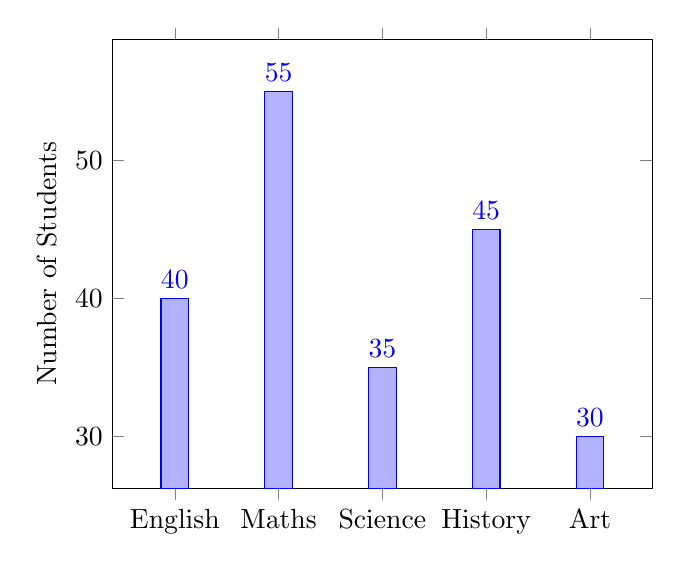
\begin{tikzpicture}
\begin{axis}[
    ybar,
    enlargelimits=0.15,
    ylabel={Number of Students},
    symbolic x coords={English,Maths,Science,History,Art},
    xtick=data,
    nodes near coords,
    nodes near coords align={vertical},
]
\addplot coordinates {(English,40) (Maths,55) (Science,35) (History,45) (Art,30)};
\end{axis}
\end{tikzpicture}

\item What subject has the most students?
\item What is the total number of students in all subjects?
\item 

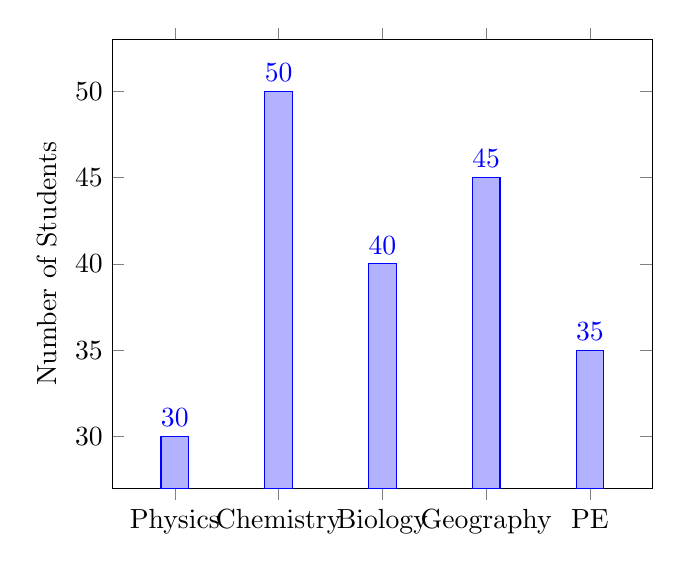
\begin{tikzpicture}
\begin{axis}[
    ybar,
    enlargelimits=0.15,
    ylabel={Number of Students},
    symbolic x coords={Physics,Chemistry,Biology,Geography,PE},
    xtick=data,
    nodes near coords,
    nodes near coords align={vertical},
]
\addplot coordinates {(Physics,30) (Chemistry,50) (Biology,40) (Geography,45) (PE,35)};
\end{axis}
\end{tikzpicture}

\item What subject has the fewest students?
\item What is the total number of students in all subjects?
\item 

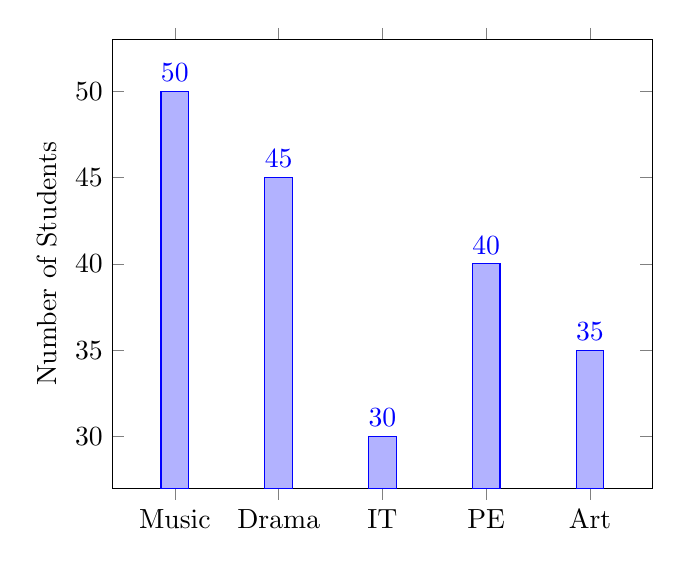
\begin{tikzpicture}
\begin{axis}[
    ybar,
    enlargelimits=0.15,
    ylabel={Number of Students},
    symbolic x coords={Music,Drama,IT,PE,Art},
    xtick=data,
    nodes near coords,
    nodes near coords align={vertical},
]
\addplot coordinates {(Music,50) (Drama,45) (IT,30) (PE,40) (Art,35)};
\end{axis}
\end{tikzpicture}

\item What subject has the most students?
\item What is the total number of students in all subjects?
\end{enumerate}

\section*{Clock and Time}

\begin{enumerate}
\setcounter{enumi}{38}
\item What time will it be 3 hours after 2:00 PM?
\item If it is now 10:30 AM, what was the time 2 hours and 30 minutes ago?
\item A movie starts at 6:45 PM and lasts for 2 hours and 15 minutes. At what time does the movie end?
\item If a train departs at 11:00 AM and arrives at 3:00 PM, how long is the train journey?
\item How many minutes are there from 2:00 PM to 4:30 PM?
\end{enumerate}

\section*{Distance}

\begin{enumerate}
\setcounter{enumi}{43}
\item If John walks at a speed of 3 km/h, how far will he travel in 2 hours?
\item Mary cycles at a speed of 10 km/h. How far does she cycle in 30 minutes?
\item If a car travels 80 km in 1 hour, what is its speed in km/h?
\item A bus travels 60 km in 2 hours. What is its speed in km/h?
\item Peter runs at a speed of 5 km/h. How long does it take him to run 15 km?
\end{enumerate}

\section*{Pie Charts}

\begin{enumerate}
\setcounter{enumi}{48}
\item
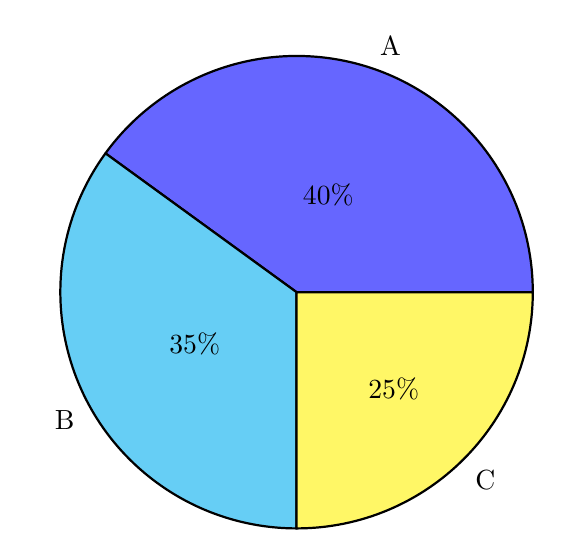
\begin{tikzpicture}
\pie{40/A, 35/B, 25/C}
\end{tikzpicture}

What percentage is category B?

\item 
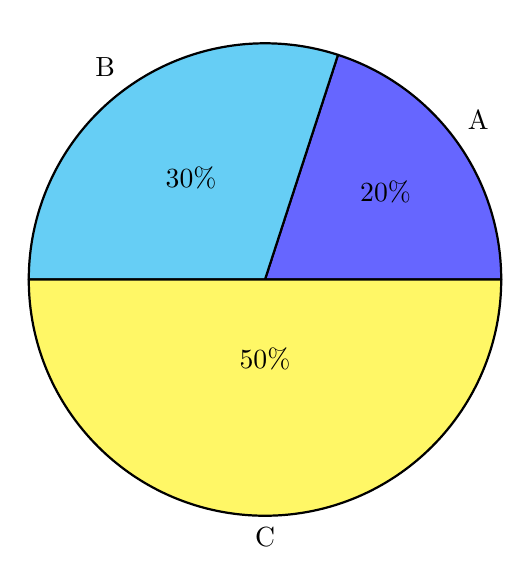
\begin{tikzpicture}
\pie{20/A, 30/B, 50/C}
\end{tikzpicture}

What percentage is category C?

\item 
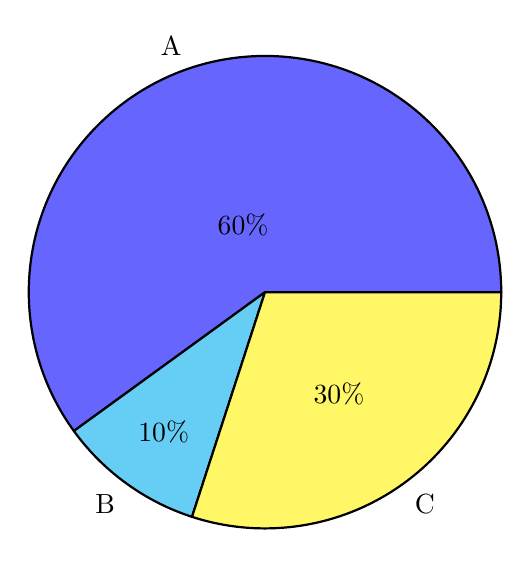
\begin{tikzpicture}
\pie{60/A, 10/B, 30/C}
\end{tikzpicture}

What percentage is category A?

\item 
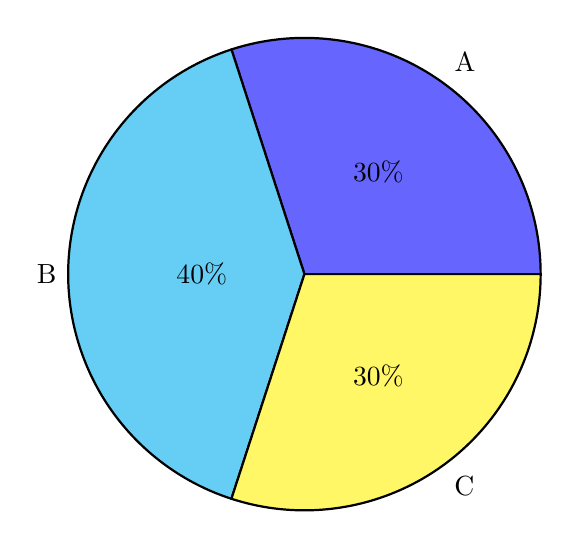
\begin{tikzpicture}
\pie{30/A, 40/B, 30/C}
\end{tikzpicture}

What percentage is category B?

\item 
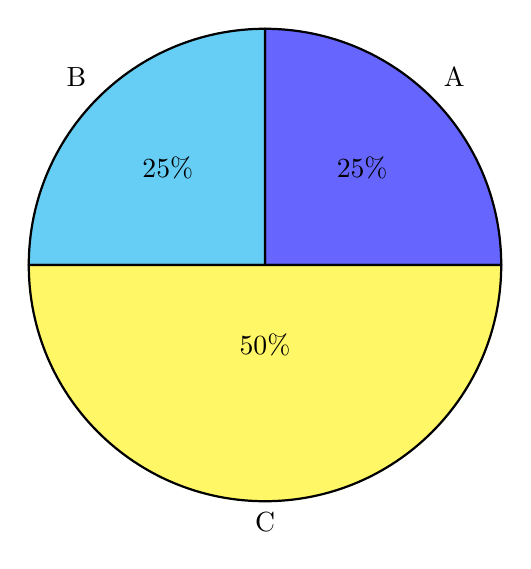
\begin{tikzpicture}
\pie{25/A, 25/B, 50/C}
\end{tikzpicture}

What percentage is category C?
\end{enumerate}

\end{document}
